\section{Development}\label{sec:dev}

  \subsection{Plugin Systems}\label{sec:dev-plugins}

    The software application that OpenDCS aims to replace uses a plugin system
    built using the GObject library gmodule-2.0. GModule and related classes
    provide a portable method for dynamically loading plugins, but it would
    require a large amount of effort to continue using this approach to address
    one of the key requirements that was identified. In early discussions that
    were had about requirements and given in Section~\ref{sec:req-sh} as \#9 of
    Table~\ref{tab:requirements}, the end user ``Must be able to develop plugins
    in Python as well as C/Vala''. While this is possible using GModule, it was
    identified by early research that doing so would be difficult, and has
    already been accomplished in another library called Libpeas. This is what
    will be used for the plugin systems incorporated in the various services.

    Libpeas is a gobject-based plugins engine, and is targetted at giving every
    application the chance to assume its own extensibility~\cite{Libpeas2016}.
    Its features include programming support for C, and Vala by extension,
    Python, and Lua so it is appropriate to address our requirement.

    More information on developing and installing Libpeas plugins is given in
    Section~\ref{sec:inst}.

  \subsection{GNU Build System}\label{sec:dev-ac}

    The GNU build system is made up of a many components, the most important of
    which are Automake, Autoconf, Gnulib, and Libtool. Files that make up this
    type of build system define a set of rules to build the files in a package
    \cite{Automake2014}. Figure~\ref{fig:dev-ac-comp} shows the basic components
    of an Autotools build system and how certain necessary input files result in
    a \texttt{Makefile} that is the recipe required to build a package. The two
    files that are required as input to this type of build system are
    \texttt{configure.ac} and \texttt{Makefile.am}, with \texttt{autoconf} and
    \texttt{automake} these files are used to produce the \texttt{configure}
    script which defines how to create the corresponding \texttt{Makefile} that
    is used with the program \texttt{make} which is the command that many expect
    to be able to call on a source package to generate a set of libraries and
    executables.

    In OpenDCS the build system is used for a variety of purposes, it defines
    binary and library version numbers, ensures that the necessary applications
    to compile are installed, to control compilation which allows for the
    inclusion of non-essential components or the exclusion of components to
    simplify builds, and to manage compiler variables including \texttt{CFLAGS}
    and \texttt{LIBS}. As it is a desired requirement of this project to be able
    to generate builds for a variety of Linux variants this type of build system
    is essential. While other systems are available, for example \texttt{CMAKE}
    and \texttt{Meson}, the developer has the most knowledge of the GNU build
    system.

    \begin{figure}[H]
      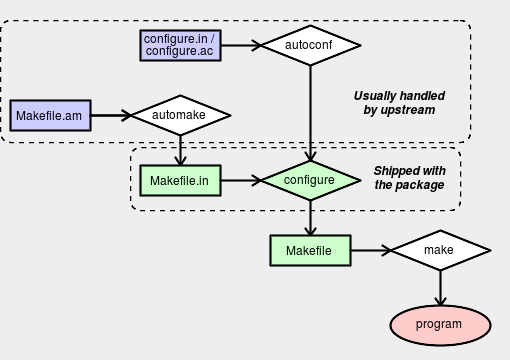
\includegraphics[width=0.8\textwidth,center]{figures/development/autotools-components}
      \caption{Basic Overview of the Autotools Components}\label{fig:dev-ac-comp}
    \end{figure}

    A standardized workflow that is generally understood and accepted by many
    users of Unix based systems is given here:

    \begin{lstlisting}
      git clone https://git.coanda.local:open-dcs/dcs.git
      cd dcs
      ./autogen.sh
      make
      sudo make install
    \end{lstlisting}

    More information on specifics about controlling compilation and installation
    of this project are given in Section~\ref{sec:inst}.

  \subsection{REST APIs}\label{sec:rest}

    A high level overview of the RESTful APIs provided by the services is given
    here, these add a method of interoperability among these and other web
    services that want to communicate with them. In most cases this means using
    the common HTTP verbs GET, POST, PUT, and DELETE as operations.

    \subsubsection{Common to All Services}\label{sec:rest-common}

      This section describes the common APIs for services that contain
      networking objects. Each service with have dedicated publishing,
      subscribing, requesting, and replying sockets where necessary to function
      as intended but they will also be capable of having additional socket
      types configured at runtime to add functionality and leave future options
      open for concepts like proxies and brokers.

      \large{\textbf{Publishers}}

      \begin{table}[H]
        \centering
        \begin{tabular}{p{3in} p{3in}}
          \toprule
          \emph{Resource} & \emph{Description} \\ [0.5ex]
          \midrule
          GET /api/net/publishers & List all publishers \\
          GET /api/net/publishers/:id & Show a publisher \\
          POST /api/net/publishers/:id & Add a publisher \\
          PUT /api/net/publishers/:id & Update a publisher \\
          DELETE /api/net/publishers/:id & Remove a publisher \\
          \bottomrule
        \end{tabular}
        \caption{API for the Publishers in Services}\label{tab:rest-common-pub}
      \end{table}

      \large{\textbf{Subscribers}}

      \begin{table}[H]
        \centering
        \begin{tabular}{p{3in} p{3in}}
          \toprule
          \emph{Resource} & \emph{Description} \\ [0.5ex]
          \midrule
          GET /api/net/subscribers & List all subscriber \\
          GET /api/net/subscribers/:id & Show a subscriber \\
          POST /api/net/subscribers/:id & Add a subscriber \\
          PUT /api/net/subscribers/:id & Update a subscriber \\
          DELETE /api/net/subscribers/:id & Remove a subscriber \\
          \bottomrule
        \end{tabular}
        \caption{API for the Subscribers in Services}\label{tab:rest-common-sub}
      \end{table}

      \large{\textbf{Requesters}}

      \begin{table}[H]
        \centering
        \begin{tabular}{p{3in} p{3in}}
          \toprule
          \emph{Resource} & \emph{Description} \\ [0.5ex]
          \midrule
          GET /api/net/requesters & List all requesters \\
          GET /api/net/requesters/:id & Show a requester \\
          POST /api/net/requesters/:id & Add a requester \\
          PUT /api/net/requesters/:id & Update a requester \\
          DELETE /api/net/requesters/:id & Remove a requester \\
          \bottomrule
        \end{tabular}
        \caption{API for the Requesters in Services}\label{tab:rest-common-req}
      \end{table}

      \large{\textbf{Repliers}}

      \begin{table}[H]
        \centering
        \begin{tabular}{p{3in} p{3in}}
          \toprule
          \emph{Resource} & \emph{Description} \\ [0.5ex]
          \midrule
          GET /api/net/repliers & List all repliers \\
          GET /api/net/repliers/:id & Show a replier \\
          POST /api/net/repliers/:id & Add a replier \\
          PUT /api/net/repliers/:id & Update a replier \\
          DELETE /api/net/repliers/:id & Remove a replier \\
          \bottomrule
        \end{tabular}
        \caption{API for the Repliers in Services}\label{tab:rest-common-rep}
      \end{table}

    \subsubsection{Data Acquisition Service}\label{sec:rest-daq}

      \large{\textbf{Devices}}

      \begin{table}[H]
        \centering
        \begin{tabular}{p{3in} p{3in}}
          \toprule
          \emph{Resource} & \emph{Description} \\ [0.5ex]
          \midrule
          GET /api/daq/devices & List all devices \\
          GET /api/daq/devices/enabled & List all enabled devices \\
          GET /api/daq/devices/:id & Show a device \\
          POST /api/daq/devices/:id & Enable a device \\
          PUT /api/daq/devices/:id & Update a device \\
          DELETE /api/daq/devices/:id & Disable a device \\
          \bottomrule
        \end{tabular}
        \caption{API for the DAQ Service Devices}\label{tab:rest-daq-dev}
      \end{table}

      \large{\textbf{Sensors}}

      \begin{table}[H]
        \centering
        \begin{tabular}{p{3in} p{3in}}
          \toprule
          \emph{Resource} & \emph{Description} \\ [0.5ex]
          \midrule
          GET /api/daq/sensors & List all sensors \\
          GET /api/daq/sensors/:id & Show a sensor \\
          POST /api/daq/sensors/:id & Add a sensor \\
          PUT /api/daq/sensors/:id & Update a sensor \\
          DELETE /api/daq/sensors/:id & Remove a sensor \\
          \bottomrule
        \end{tabular}
        \caption{API for the DAQ Service Sensors}\label{tab:rest-daq-sensor}
      \end{table}

      \large{\textbf{Signals}}

      \begin{table}[H]
        \centering
        \begin{tabular}{p{3in} p{3in}}
          \toprule
          \emph{Resource} & \emph{Description} \\ [0.5ex]
          \midrule
          GET /api/daq/signals & List all signals \\
          GET /api/daq/signals/:id & Show a signal \\
          POST /api/daq/signals/:id & Add a signal \\
          PUT /api/daq/signals/:id & Update a signal \\
          DELETE /api/daq/signals/:id & Remove signal \\
          \bottomrule
        \end{tabular}
        \caption{API for the DAQ Service Signals}\label{tab:rest-daq-signal}
      \end{table}

      \large{\textbf{Ports}}

      \begin{table}[H]
        \centering
        \begin{tabular}{p{3in} p{3in}}
          \toprule
          \emph{Resource} & \emph{Description} \\ [0.5ex]
          \midrule
          GET /api/daq/ports & List all ports \\
          GET /api/daq/ports/:id & Show a port \\
          POST /api/daq/ports/:id & Add a port \\
          PUT /api/daq/ports/:id & Update a port \\
          DELETE /api/daq/ports/:id & Remove a port \\
          \bottomrule
        \end{tabular}
        \caption{API for the DAQ Service Ports}\label{tab:rest-daq-port}
      \end{table}

    \subsubsection{Data Logging Service}\label{sec:rest-log}

      \large{\textbf{Backends}}

      \begin{table}[H]
        \centering
        \begin{tabular}{p{3in} p{3in}}
          \toprule
          \emph{Resource} & \emph{Description} \\ [0.5ex]
          \midrule
          GET /api/log/backends & List all backends \\
          GET /api/log/backends/:id & Show a backend \\
          POST /api/log/backends/:id & Enable a backend \\
          PUT /api/log/backends/:id & Update a backend \\
          DELETE /api/log/backends/:id & Disable a backend \\
          \bottomrule
        \end{tabular}
        \caption{API for the Log Service Backends}\label{tab:rest-log-backend}
      \end{table}

      \large{\textbf{Logs}}

      \begin{table}[H]
        \centering
        \begin{tabular}{p{3in} p{3in}}
          \toprule
          \emph{Resource} & \emph{Description} \\ [0.5ex]
          \midrule
          GET /api/log/logs & List all logs \\
          GET /api/log/logs/:id & Show a log \\
          POST /api/log/logs/:id & Add a log \\
          PUT /api/log/logs/:id & Update a log \\
          DELETE /api/log/logs/:id & Remove a log \\
          \bottomrule
        \end{tabular}
        \caption{API for the Log Service's Configured Logs}\label{tab:rest-log-logs}
      \end{table}

      \large{\textbf{Log Columns}}

      \begin{table}[H]
        \centering
        \begin{tabular}{p{3in} p{3in}}
          \toprule
          \emph{Resource} & \emph{Description} \\ [0.5ex]
          \midrule
          GET /api/log/columns & List all columns \\
          GET /api/log/columns/:id & Show a column \\
          POST /api/log/columns/:id & Add a column \\
          PUT /api/log/columns/:id & Update a column \\
          DELETE /api/log/columns/:id & Remove a column \\
          \bottomrule
        \end{tabular}
        \caption{API for the Log Service's Configured Data Columns}\label{tab:rest-log-columns}
      \end{table}

      \large{\textbf{Data Query}}

      \begin{table}[H]
        \centering
        \begin{tabular}{p{3in} p{3in}}
          \toprule
          \emph{Resource} & \emph{Description} \\ [0.5ex]
          \midrule
          GET /api/log/query/:id & Query a log \\
          \bottomrule
        \end{tabular}
        \caption{API for Log Service Queries}\label{tab:rest-log-query}
      \end{table}

    \subsubsection{Process Control Service}\label{sec:rest-control}

      \large{\textbf{Feedback Controllers}}

      \begin{table}[H]
        \centering
        \begin{tabular}{p{3in} p{3in}}
          \toprule
          \emph{Resource} & \emph{Description} \\ [0.5ex]
          \midrule
          GET /api/control/controllers & List all controllers \\
          GET /api/control/controllers/:id & Show a controller \\
          POST /api/control/controllers/:id & Enable a controller \\
          PUT /api/control/controllers/:id & Update a controller \\
          DELETE /api/control/controllers/:id & Disable a controller \\
          \bottomrule
        \end{tabular}
        \caption{API for the Process Control Service Feedback Controllers}\label{tab:rest-control-controllers}
      \end{table}
